\documentclass[a4paper]{article}
\usepackage[utf8]{inputenc} 
\usepackage[danish]{babel} 

\usepackage{amsmath}
\usepackage{amsfonts}
\usepackage{amssymb}
\usepackage{ulem}
\usepackage{verbatim}
\usepackage{graphicx}
\usepackage{xcolor}
\usepackage{marvosym}

\newcommand*{\mybox}[2]{\colorbox{#1!30}{\parbox{.98\linewidth}{#2}}}
\newcommand{\setR}{\mathbb{R}} 
\newcommand{\setF}{\mathbb{F}} 
\newcommand{\setN}{\mathbb{N}} 
\newcommand{\pder}[2][]{\frac{\partial#1}{\partial#2}}
\newcommand{\RNum}[1]{\uppercase\expandafter{\romannumeral #1\relax}}

\newcommand*{\titleGM}{\begingroup % Create the command for including the title page in the document
	\hbox{ % Horizontal box
		\hspace*{0.2\textwidth} % Whitespace to the left of the title page
		\rule{1pt}{\textheight} % Vertical line
		\hspace*{0.05\textwidth} % Whitespace between the vertical line and title page text
		\parbox[b]{0.75\textwidth}{ % Paragraph box which restricts text to less than the width of the page
			
			{\noindent\Huge\bfseries PoP \\[0.5\baselineskip] }\\[2\baselineskip] % Title
			{\large \textit{Ugeopgave 1}}\\[4\baselineskip] % Tagline or further description
			{\Large \textsc{Beate Berendt Søegaard}}\\ % Author name
			{\Large \textsc{Mathias Larsen}}\\ % Author name
			{\Large \textsc{Simon Rotendahl}} % Author name
			
			\vspace{0.5\textheight} % Whitespace between the title block and the publisher
			{\noindent Datalogi}\\[\baselineskip] \today% Publisher and logo
		}}
		\endgroup}
	
%\title{Navnet på faget  \\ \Large Aflevering}
%\author{Beate B. Søegaard}
\begin{document}
%\maketitle
%\tableofcontents
\titleGM % This command includes the title page
\section*{1.1: Et Dybfølt Program (DupiDupi) af AMG}
Vi følte dyb i vores hjerter at vi skulle skabe et program, hvori en kat skulle kunne løbe rundt og spise kager. Dertil skulle der også være en hund inkluderet, som ville blive spist til sidst af katten.\\
\begin{figure}[h]
	\centering
	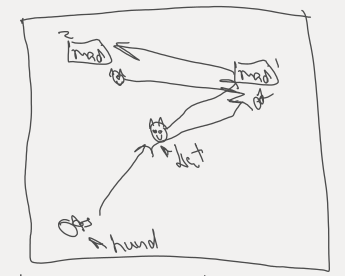
\includegraphics[scale=0.8]{kladde_ide.png}
	\caption{Skitse af vores ide}
	\label{fig: skitse}
\end{figure}

For at få vores program til, at virke måtte vi dog bruge 
\includegraphics[scale=0.5]{flag.png} istedet for 
\includegraphics[scale=0.5]{sprite.png}.
Det blev vi nødsaget til, da alle figure skulle \textit{starte} samtidigt.\\
Skærmbilleder af Dupi Dupi,\\

\includegraphics[scale=0.5]{screen_1.png}

\includegraphics[scale=0.5]{screen_3.png}


\newpage
\section*{1.2: Popping Cats af AMG}
Spillet er inspireret af \textit{Space Invaders}. Idéen med spillet er, at du spiller en drage som skyder efter kattene, der kommer ind fra siden, hvor en dødsanimation dukker op når en kat er ramt. Spilleren taber hvis dragen bliver ramt/rammer en af kattene. Spilleren vinder forsåvidt ikke, men får derimod to score. En for tid for overlevelse og en for hvor mange katte der er blevet "poppet".
\begin{figure}[h]
	\centering
	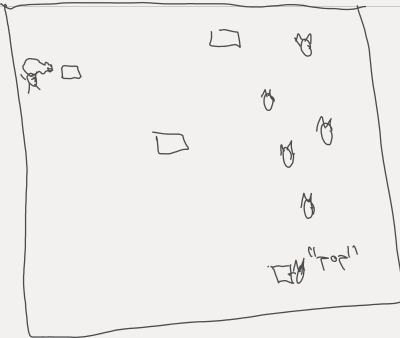
\includegraphics[scale=0.8]{kladde_spil.png}
	\caption{Skitse af vores gameplay}
	\label{fig: skitse_spil}
\end{figure}

Skærmbilleder af Popping Cats,\\
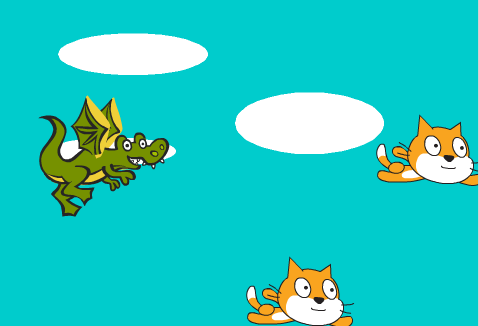
\includegraphics[scale=0.5]{screen_game0.png}
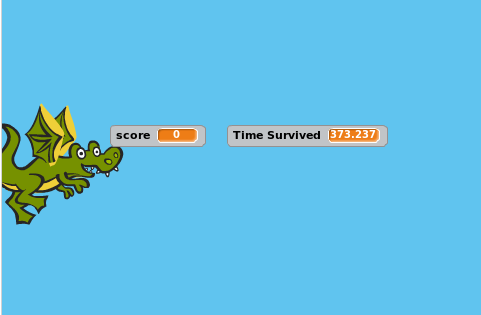
\includegraphics[scale=0.5]{screen_game1.png}

Der er en fejl i spillet. Når du rammer bunden af en kat bliver skudet ikke ødelagt, men fortsætter ind i den næste kat. Fejlen opstår enten på grund af forskellen i de to figuer er forskellige størrelser, eller at skudet ikke når at registrerer at den bliver ramt af katten.
\end{document}